\section{The experience Web} % (fold)
\label{sec:musical_experience_in_the_web}

The World Wide Web keeps one billion persons connected \cite{Comscore09} and has just turned eighteen \cite{BernersLee91}.
In its come of age, the Web has grown not just in quantity, % of users and pages, 
but most importantly in quality.
Old-fashioned media have spent years questioning the reputation of Internet as a trustworthy source \cite{Johnson04} and have been outwit. 
Internet offers worldwide information with a swiftness and a level of granularity that cannot be found in books, newspapers, radios or televisions while preserving the same accuracy \cite{Giles05}.

The power for the Internet to evolve from a limited and disregarded to a rich and outspread medium comes from enabling anyone to easily contribute to its content.
While Web publishing in the 1990s was cumbersome and expensive, nowadays a few clicks are enough to share content on the Web, with publishing services such as YouTube (video), MySpace (music) and Flickr (images) having become of public domain.

The most remarkable effect of enabling people to easily share content has been to have more people create new content.
Most blogs' writers, for instance, never had a personal diary on paper, while millions of pictures, videos, animations, stories are created on purpose to be broadcast online.
Internet provides content that would simply be unavailable or inexistent otherwise.

\subsection{A repository of personal experiences} % (fold)
\label{sub:a_repository_of_personal_experiences}

A particular type of content that has recently gained ground in the Web is \textbf{experience data}. 
This refers to data describing what people have been doing: where they have been, which songs they have played, % which movies they have watched, 
which friends they have met, and so on. Most people enjoy sharing this personal information, which explains the success of Web services such as Facebook and Twitter, where no original content is actually created.
What is shared are \emph{personal experiences}, in such a quantity that cannot be found in any other place.

Experience data from the Web grants a valuable overview of the social impact of a given content. % that cannot be found anywhere else.
An example is provided by
% \href{http://www.last.fm/music/Panic+at+the+Disco}{Panic!\;At The Disco}, 
Panic!\;At The Disco, 
a Rock band that gained online fame thanks to the `buzz' generated in the music communities MySpace and PureVolume. 
While unsigned bands typically have a reduced group of listeners in these Web sites, Panic!\;At The Disco singularly broke this rule, with more people playing their songs week after week and eventually reaching number one in MySpace's indie chart, which brought them to sign a contract and sell almost four million copies with their first album.

The lesson learnt is that knowing what many people are doing online with music is very valuable. Music labels are now aware of the importance of online experience data and more unsigned artists are reported to have been offered contracts because they had many online listeners or many `friends' (MySpace jargon for `supporters') shared with other famous musicians.
The strategical importance of collecting musical experience data from the Web is also confirmed by MySpace and Last.fm\,---\,two of the main music-driven online communities\,---\,being recently acquired by media corporations News Corp. and CBS Interactive for 580 million dollars and 280 million dollars respectively \cite{News05,Cbs07}.

% subsection a_repository_of_personal_experiences (end)

%Knowing how people experience music on the Web has become crucial. Being able to depict who is the most `hip' artist of the week, or which online social relationships hold among different bands (`people who listen to X also listen to Y') is essential for both musicians, producers and listeners. 

\subsection{Collecting music-related experiences} % (fold)
\label{sub:analysing_music_related_experiences}

Extracting music-related experience data from the Web is not easy task.
People have a hand of choices to narrate their `musical experiences' online: writing a post about a new song in a blog, reporting part of the lyrics in a forum, watching the video in YouTube, playing the audio in Last.fm, becoming friend of the band in MySpace: all these behaviours denote an interest for a song, yet they are all stored in different sites and cannot be easily aggregated. 

This is particularly true for experiences described in a \emph{textual} format.
Blog posts, for instance, can report both positive and negative music experiences (an awesome concert, a disappointing album);
to really understand what is said about music, one would have to read the whole text, filter out typo errors, identify where the music is referred to and categorise the experience.

A human could perform this process only on a small number of blog posts, certainly not on all the posts that bloggers generate daily.
On the other hand, an automatic system would have it hard to understand what a blog post is about, given the infinite quantity of languages, styles and locutions that can describe musical experiences. 

Luckily, there are musical experiences that are shared on the Web in non-textual formats and that, as such, do not require an \emph{interpretation} since they clearly imply which music a person has experienced and how.
The main format to describe songs that have been played and enjoyed is that of playlists.

% BELLA, MA NON SO DOVE METTERLA: Extracting this knowledge from the fabric of the Web is not simple, because people share their experience data online without a \emph{uniquely defined structure}. 

% subsection analysing_music_related_experiences (end)

\subsection{The value of playlists} % (fold)
\label{sub:the_value_of_playlists}

Playlists are ordered sequences of music titles.
Many persons use playlists in their digital players to specify which songs they would like to hear for a given occasion, for instance reading, programming, driving, working, waking up, going to sleep \cite{Vignoli04}.
People also create playlists that reflect a particular mood or emotion, that tell a story or are meant to be shared with friends \cite{Cunningham04}.
Playlists can be thought of as a ``collective memory'' \cite{vanDijck06} of the way in which people organise their music.

Playlists are very valuable to automatically extract experience data about music from the Web because they are are less prone to interpretation errors. Each playlist has a clear structure: a sequence of songs that a person compiled to be played together. Even ignoring the \emph{motivation} that drove someone to put songs in a certain sequence, the same effort of compiling and publishing a playlist indicates a preference for those songs.

The singularity of playlists, compared to other experience data (blog posts, album reviews, concert reports), is that playlists intrinsically bind \emph{multiple} songs and artists together. Someone compiling and sharing a playlist is not expressing an interest for a single song, but for a particular sequence of songs meant to be played in a specific order.
%
For this reason, playlists not only offer an overview of which songs or artists are more or less played, but also of which songs or artists people tend to \emph{associate}, to play together. 


% subsection the_value_of_playlists (end)

\subsection{From playlists to musical associations} % (fold)
\label{sub:from_playlists_to_musical_associations}

When people compile playlists, they include songs that are meant to be played together for some purpose. 
If two songs or artists appear in many playlists by many different authors, then it makes sense to assess that those songs or artists are \emph{associated}.

The purpose of this chapter is to define a measure of \textbf{musical association} to estimate how much two songs or artists `go well together' based on their playlist co-occurrences.
%
The approach consists in retrieving playlists from Internet and analysing the co-occurrences of songs and artists in such playlists to determine how much they go well together. %, according to the people's experience.

The hypothesis is that if any association (cultural, social, or acoustic) exists between two songs or artists, this can be automatically revealed observing how a multitude of people have organised their music in playlists shared on the Web.
%
Playlists hide valuable personal experiences; this chapter shows how these experiences can be extracted and musical associations uncovered.


% subsection from_playlists_to_musical_associations (end)

% section musical_experience_in_the_web (end)

\section{Previous work} % (fold)
\label{sec:previous_works2}

The approach described in this chapter explains how to reuse experience data included in playlists to assess a measure of musical association between songs and artists.
This section reviews previous work addressed to estimate musical associations among musical objects, with a particular emphasis on methods that exploit data retrieved from the Web.


\subsection{Co-occurrence analysis} % (fold)
\label{sub:co_occurrence_analysis}

Some researchers assume that playlists contain ``similar music'' \cite{Logan03} and that, if two songs are contiguously one after the other in a playlist, it somehow makes sense to play them in this order \cite{Andric06}.
Although this assumption may not hold for one playlist, applying this hypothesis to a large data set of playlists implies that associated songs can be discovered when they co-occur in many playlists.

Identifying relevant \emph{co-occurrences} of items in a series of events is a common issue in unsupervised learning \cite{Hofmann98}.
Co-occurrence analysis has been applied not only to identify associated songs from a set of playlists, but also to find  maximal frequent sequences in text \cite{Ahonen99}, to discover interesting episodes in the alarm flow of telecommunications networks \cite{Mannila97}, to gather knowledge about DNA sequences \cite{Wang97} or to learn Web navigation models \cite{Nakagawa03}.

The main benefit of co-occurrence analysis is that it allows to state whether two resources are associated or not, not because of some intrinsic content, but because of they way objects are organised.
%
In the case of music, assessing that two songs are associated because they co-occur in many playlists is a way to reveal the ``wisdom of the crowd'' \cite{Surowiecki04}, the way in which songs are most associated by people in their activities.

The basic idea of co-occurrence analysis is that the higher the \emph{number} of playlists where two songs co-occur, the higher their association.
As \citet{Andric06} first noticed, the \emph{order} in which songs appear in playlists is another important property that should be tracked to determine their association.
\citet{Ragno05} suggested that the \emph{distance} at which songs co-occur in a playlist is also relevant: songs appearing contiguously in a playlist are more enlaced that songs divided by a certain time gap.
\citet{Pachet01} indicated how the \emph{popularity} of each song is also fundamental in the co-occurrence analysis since popular songs tend to occur in playlists with many other songs, independently of any real musical association.

Co-occurrence analysis can be performed at different level of \emph{granularity}, focusing either on the co-occurrences of songs, of albums, or of artists.
\citet{Hauver01} suggested that, since songs performed by the same artist are often similar, working at the level of artists can be useful, especially when the data set is small or sparse.

% subsection co_occurrence_analysis (end)

\subsection{Playlists} % (fold)
\label{sub:retrieving_playlists}

To analyse co-occurrences of songs in a large set of playlists, first many playlists compiled by different persons need be retrieved from the Web.
%
Playlists can be found in millions throughout Web pages of different countries and cultures.
Many authors publish their personal playlists online, either directly from their music players (e.g., Apple iTunes, Spotify) or inside online communities, the most popular being Imeem, Playlist.com, FIQL, Last.fm, MusicStrands, SonicSwap, Art Of The Mix, Plurn and UpTo11.

Although there is no unique way to distribute playlists online, the most common representation is the XML Shareable Playlist Format (XSPF) \cite{XSPF06} that specifies, for each song in the playlist, its title, artist name, album name, song length and location.


Sometimes a song can appear in different databases with different titles, and this can make it difficult to compare playlists shared among different communities. 
For instance the song `The Bitter End' (Placebo) is represented as `The Bitter End' (Placebo) in Last.fm, as `Bitter End, The' (Placebo (Pop)) in MusicStrands, and as `Placebo-Bitter End' () in Plurn.
%
The main reason for this misalignment is that, although the music industry has defined an ISO standard music title reference\,---\,the ISRC code \cite{ISRC03}\,---\,this is usually not used in existing information database, as pointed out by \citet{Pachet01}.

Possible solutions to univocally identify music titles are to either use audio fingerprinting \cite{Cano05}, music ontology matching \cite{Raimond07b} or to query large online public music databases such as Musicbrainz.

% subsection retrieving_playlists (end)

\subsection{Other Web-based musical experience} % (fold)
\label{sub:other_web_based_musical_experience}

Playlists are not the only type of online data that can be analysed to assess associations between songs and artists.

\citet{Cohen00} first suggested that co-occurrences of musical artists in Web \emph{search results} reflect the way in which people associate artists in the music domain.
On the same line, \citet{Whitman02} described a method which first queries search engines for pages related to an artist, next extracts natural language features from these pages to produce a summary description of the artist, and finally uses this description to compute similarity between artists.
\citet{Zadel04} proposed to combine Web services from Amazon and Google to generate pools of potentially related artists and use Web search result counts to assess their actual relatedness.
\citet{Schedl06b} also employed Web services to search for combinations of artists’ names with keywords like `music', `genre', `style'.

The main limitation of these methods, as observed by \citet{Levy07}, is that they are inherently noisy.
Firstly, the pages retrieved from a search engine are not guaranteed to be relevant (e.g., the word `Prince' appears in many pages not related to the artist known as Prince).
Secondly, the simple fact of appearing together in a Web page does not guarantee that two musical objects are positively associated (e.g., online shops can present their entire music catalogue on the same page). %, from Acid Jazz to Zulu music).
Thirdly, noise further multiplies if search engines are used to find songs rather than artists.
In general, the textual nature of this approach makes it difficult to guarantee that the results are indeed representative of any association.

An alternative to Web search analysis is to crawl Internet for entire music collections.
\citet{Brown01} designed a system by which users upload their entire music collections to a centralised server, where co-occurrences of songs and artists are calculated.
\citet{Logan03} proposed to exploit OpenNap, a popular music sharing service, to obtain personal music collections and infer association between artists under the assumption that artists co-occurring in someone's collection have a better-than-average chance of being similar. 
%
These methods are not based on text analysis, thus remove the noise problems related to Web search.
The main drawback is that only a limited number of users share their whole music collections on the Internet. % , and the fact that no order, size, etc.

% subsection other_web_based_musical_experience (end)

\subsection{Other ways to assess musical associations} % (fold)
\label{sub:other_ways_to_assess_musical_associations}

Other approaches not based on experience data can be used to assess whether two songs go well together or not. 
%
One option is to analyse intrinsic content and deduce that two songs go well together when they have either similar symbolic representations, similar lyrics or similar acoustic features.
These hypotheses, however, are quite strong, since people often relate two songs for cultural and social motivations that cannot be revealed by a content-based analysis.
A different option is to ask for experts' opinion. 

\subsubsection{Symbolic analysis} % (fold)
\label{ssub:signal_analysis}

%The content of a song can be described in terms of symbolic data, such as the timing and position of each note, their pitch, instrument, duration, chord, et cetera.
\citet{Chen01} first proposed to identify associated songs by comparing their symbolic information in the form of six different features: mean and standard deviation of the pitch values, pitch density, pitch entropy, tempo degree and loudness.
\citet{Kuo02} proposed to identify associated songs comparing their chords.

The main limitation of these approaches is the requirement of a MIDI \cite{MIDI96} representation for each song which is often unavailable and, in the case of polyphonic songs, hardly conveys information about representative tracks.
Symbolic information might also be obtained from the score of a theme but, as \citet{Logan03} observed, only a small subset of music has good-quality machine-readable score descriptions available and automatic transcription becomes difficult and error-prone for anything other than monophonic music.
% subsubsection signal_analysis (end)


\subsubsection{Textual analysis} % (fold)
\label{ssub:lyrics_analysis}

A different content-based representation for song is by terms of textual context.
\citet{Kaji05} and \citet{Mahedero05} first proposed to represent songs as vectors of keywords extracted from the lyrics and to measure their association comparing their weighted cosine coefficients.

Other lyrics-based approaches were proposed in the works by \citet{Kleedorfer08} and \citet{Mayer08}:
the former uses text mining techniques to identify topic clusters and considers songs falling under the same topic (loss, family, love, etc.) as associated;
the latter identifies associated songs based on their rhyme type, part-of-speech and statistic features (e.g., number of `AABB' rhymes, exclamation marks, articles).

The limitation of these approaches is that they only work for music containing lyrics.
Moreover, lyrics have to be available, since automatic lyrics extraction from audio is not yet a reality \cite{Berenzweig01}.
% subsubsection lyrics_analysis (end)

\subsubsection{Acoustic analysis} % (fold)
\label{ssub:acoustic_analysis}

The most common content-based representation for music is through a series of acoustic features extracted from the audio signal.
\citet{Aucouturier02b} suggested that associated songs can be identified based on their global timbral quality.
A common technique to compute timbral quality is by representing a song in terms of clusters of Mel Frequency Cepstrum Coefficients (MFCCs) \cite{Aucouturier04}, a measure of spectral shape historically used as a feature for speech recognition: songs are cut into short overlapping frames, a feature vector made of several MFCCs is computed for each frame, a statistical model of the MFCCs' distribution is calculated and finally models are compared to identify songs that sound similar according to their timbre.
%
%[..Here add \cite{Sandler07}..]
%
Approaches based on beat and tempo analysis \cite{Tzanetakis02} and singing voice segmentation \cite{Berenzweig02} have also been investigated to identify songs that sound similar.

Although these unsupervised approaches can interestingly spot out associated songs with different cultural background, or from different genres, they all present a main drawback: scalability.
The actual songs (audio content) have to be available to perform the analysis, which limits the results to the music available to each researcher.
% subsubsection acoustic_analysis (end)

\subsubsection{Expert analysis} % (fold)
\label{ssub:expert_based_smoothness}

The task to identify associated songs is faced by any disc jockey required to play a sequence of songs that flow smoothly one after the other, for instance in a discotheque, a radio, or a recorded music compilation.
Analysing the way in which professional DJs select and order songs in their sets can convey valuable knowledge about associated songs.

\citet{Weiss00} presented a comprehensive analysis on how professional DJs select in real time which songs to play, underlying how the overall flow and movement between different kinds of music is an important part of the experience.
\citet{Gates06} also interviewed several DJs about the way in which musical sequences are prepared.
%[DJ University] also reports common techniques to order songs among DJs, such as avoiding to play ``more than two fast songs of any given music group if you are getting little or no dance response'' or ``to play a variety that will please the majority of people, most of the time''.

The expertise of DJs was employed by \citet{Ragno05} to identify smooth musical transitions. 
The authors retrieved expertly authored streams from Nielsen Broadcasting Data (a service monitoring the music broadcast in more than 1,600 radio stations, satellite radio and cable music channels), translated them to undirected graphs connecting adjacent songs in each stream, and then used this knowledge to to generate smooth musical playlists.

The main limitation of expert-based analysis is that musical sequences compiled by professionals are scarcely available or are subject to a fee, as for the Nielsen data set.
% subsubsection expert_based_smoothness (end)


% subsection other_ways_to_assess_musical_associations (end)

% section previous_works2 (end)


%\section{Problem description} % (fold)
%\label{sec:problem_description}


\section{Co-occurrence analysis of social data} % (fold)
\label{sec:co_occurrence_analysis5}

The purpose of this section is to define a musical association degree that measures \emph{how much} any two songs or artists go well together in sequence.

A social-based approach is employed: first a large set of playlists compiled by thousands of users is retrieved from the Internet, then these playlists are analysed and the most frequently co-occurrent songs and artists identified.

Let $\mathcal{C}$ be the set of songs appearing in the retrieved playlists; the goal of this section is to define a \textbf{musical association} degree $s: \mathcal{C}^2 \to [0,1]$ that measures how much any two songs go well in sequence. The higher the value $s(X,Y)$, the more two songs $X, Y \in \mathcal{C}$ go well together in a musical sequence.

\subsection{Conditional probability} % (fold)
\label{sub:conditional_probability}

Let $c(X) \in \mathbb{N}$ and $c(Y) \in \mathbb{N}$ be the \textbf{occurrence counts} of song $X$ and $Y$, that is, the number of playlists where each song occurs;
let $d(X,Y,1) \in \mathbb{N}$ be the number of \textbf{contiguous sequential patterns}, that is, the number of times $Y$ occurs in a playlist immediately after $X$; 
let
\begin{equation*}
        N = \sum_{X,Y \in \mathcal{C}} d(X,Y,1)
\end{equation*}
be the total number of contiguous sequential patterns.
%
The value 
\begin{equation}
    \frac{d(X,Y,1)}{c(X)}    
\label{eq:conditional_probability}
\end{equation}
is the conditional probability to find $Y$ as the following element in a playlist containing $X$.
The conditional probability \eqref{eq:conditional_probability} looks like a good indicator of the association from $X$ to $Y$: 
if people tend to play song $Y$ right after song $X$, then the value of \eqref{eq:conditional_probability} is high, otherwise the value is low.
%
The problem is that this measure is biased by the popularity of $Y$: it may return a high value because song $Y$ occurs in many playlists, rather than because $X$ and $Y$ are indeed associated.

For example, let $X$, $Y$ and $Z$ be three songs with respective occurrence counts $c(X) = 100$, $c(Y) = 60$, and $c(Z) = 5$, and such that $d(X,Y,1) = 6$ and $d(X,Z,1) = 4$. 
The conditional probabilities to find either $Y$ or $Z$ in a playlist after song $X$ are:
\begin{equation*}
  \frac{d(X,Y,1)}{c(X)} = 0.06 > \frac{d(X,Z,1)}{c(X)} = 0.04%\,,
\end{equation*}
which show that $Y$ occurs more frequently (6 times) than $Z$ (4 times) as the next song of a sequence after $X$. 
Yet, $Y$ is very popular and occurs after $X$ only in \emph{6 out of 60} sequences where it appears (10\%), 
while $Z$ is less popular and still occurs after $X$ in \emph{4 out of 5} sequences where $Z$ appears (80\%).

To counter-effect the bias given by the over-popularity of a song ($Y$ in the previous example), the conditional probability \eqref{eq:conditional_probability} is multiplied by a weight inversely related to the popularity of the song, as follows:
\begin{equation}\label{eq:weighted_probability}
 \frac{d(X,Y,1)}{c(X)}\left(1-\frac{c(Y)}{N}\right)^\beta 
\end{equation}
where $\beta \in [0,1]$ is a parameter tuned to punish more or less the bias given by the individual occurrence count. 
Note that when $\beta = 0$, the function is identical to \eqref{eq:conditional_probability}. %, and that for every value of $\beta$, the function yields values in the interval $[0,1]$, since $d(X,Y,1) \leqslant c(X)$ and $d(X,Y,1) \leqslant c(Y)$ by definition.

%\subsection{Expanding co-occurrence analysis} % (fold)
%\label{sub:expanding_co_occurrence_analysis}

The measure \eqref{eq:weighted_probability} yields positive values for every pair of songs $X$ and $Y$ that appear in playlists exactly one after the other.
There are other pairs of songs that can be considered associated, albeit to a smaller degree. 
Firstly, two songs $X$ and $Y$ that co-occur in many playlists \emph{separated} by other songs (e.g., $X$ followed by a song, followed by $Y$) can be seen as associated, since people tend to play them together often, although not exactly one after the other.
Secondly, two songs $X$ and $Y$ that co-occur in playlists in the inverse order ($X$ after $Y$ rather than $X$ before $Y$) can also be seen as associated.
Hereafter these cases are integrated in the measure \eqref{eq:weighted_probability}.

% In Section () I will evaluate this hypothesis on a real data set, to verify whether this improves the quality of musical associations found.

% subsection conditional_probability (end)

\subsection{Distant co-occurrences} % (fold)
\label{sub:distance_of_the_occurrences}

Let $d(X,Y,D) \in \mathbb{N}$ be the number of playlists where $X$ and $Y$ co-occur at a distance $D \in \mathbb{N}^+$; for example $d(X,Y,1)$ counts the playlists where $Y$ occurs immediately after $X$, $d(X,Y,2)$ counts the playlists where $Y$ occurs after $X$ separated by one song, %$d(X,Y,-1)$ counts the playlists where $Y$ occurs immediately before $X$, 
and so on.

If two songs $X$ and $Y$ occur in playlists not only contiguously but also separated by other songs, this is a further evidence that $X$ and $Y$ are associated.
%
While \eqref{eq:weighted_probability} considered only co-occurrences of $X$ and $Y$ at distance 1, the following formula estimates the association considering co-occurrences at a generic distance $J$:
\begin{equation}
    t_J(X,Y) = \frac{d(X,Y,J)}{c(X)}\left(1-\frac{c(Y)}{N}\right)^\beta\!\!\!\!.
\end{equation}
%
Co-occurrences between $X$ and $Y$ \emph{at different distances} are aggregated by means of a linear combination that assigns more importance to closer co-occurrences, as follows:
\begin{equation}\label{eq:distance_probability}
     \sum_{J=1}^\delta \alpha_J t_J(X,Y)   
\end{equation}
where $\delta \in \mathbb{N}^+$ is the maximum distance considered and $\alpha_1, \alpha_2, \ldots, \alpha_\delta \in [0,1]$ are the degrees in which distance influences the strength of the association. These values are decreasingly ordered  ($\alpha_1 \geqslant \alpha_2 \geqslant \alpha_3 \geqslant \cdots$) to assign more importance to closer co-occurrences, and are such that $\sum_{J=1}^\delta \alpha_J = 1$.
%
Note that when $\delta = 1$ the function is identical to \eqref{eq:weighted_probability}. 
% subsection distance_of_the_occurrences (end)

\subsection{Inverse co-occurrences} % (fold)
\label{sub:order_of_the_occurrences}

%My second hypothesis is that 
If two songs $X$ and $Y$ not only occur in many playlists in this order ($X$ before $Y$), but also in the opposite order ($X$ after $Y$), this is a further evidence that $X$ and $Y$ are associated.
The following measure $t: \mathcal{C}^2 \to [0,1]$ aggregates direct and inverse co-occurrences by means of a linear combination:
\begin{equation}\label{eq:item_association}
 t(X,Y) = \sum_{J=1}^\delta \alpha_J \left[ (1-\gamma)\cdot t_J(X,Y) + \gamma\cdot t_J(Y,X)  \right]
\end{equation}
where $\gamma \in [0,0.5]$ is a parameter to take more or less into account the order of occurrence: when $\gamma = 0$ the function is identical to \eqref{eq:distance_probability}.

%Note that $t(X,Y)$ is not biased by song popularity, aggregates co-occurrences at different distances and orders, and yields values in the interval $[0,1]$. 

% subsection order_of_the_occurrences (end)

\subsection{Co-occurrences of songs with artists} % (fold)
\label{sub:expanding_to_artists}

So far, only co-occurrences among songs have been examined.
Co-occurrences between \emph{artists} are also relevant to determine whether two songs go well in sequence or not.
If a song $X$ not only co-occurs often with a song $Y$ but also with other songs by the same artist of $Y$, this is a further evidence that $X$ and $Y$ are associated.

For example, let $X$ and $Y$ be the songs `True Colors' (Cyndi Lauper) and `Holiday' (Madonna). 
If the data set of playlists is sparse, the number of playlists where $X$ and $Y$ occur together can be small and not disclose the association between the two songs. 
Observing the co-occurrences between `True Colors' and other songs by Madonna, though, can reveal that the two artists are indeed related. % and, by association, that the songs $X$ and $Y$ can go well together in sequence.

Formally, let $a(Y)$ be the artist performing song $Y$, and let $\mathcal{U}_{X,Y} = \{U\,|\,U \neq Y \wedge a(U) = a(Y) \wedge s(X,U) > 0 \}$ be the set of songs from the same artist of $Y$ that co-occur with $X$.
The following measure $u: \mathcal{C}^2 \to [0,1]$ calculates the average degree in which $X$ co-occurs with other songs by the artist of $Y$:
\begin{equation}\label{eq:song_to_artist}
	u(X,Y) = \sum_{U \in \mathcal{U}_{X,Y}}\frac{t(X,U)}{\#(\mathcal{U}_{X,Y})}
\end{equation}
where the symbol $\#$ denotes the cardinality of a set.
The higher the value of $u(X,Y)$, the more $X$ is associated with the artist $a(Y)$, the higher the evidence that $X$ and $Y$ go well together. 
%and is called the \textbf{song-to-artist association degree}.

% subsection expanding_to_artists (end)

\subsection{Co-occurrences among artists} % (fold)
\label{sub:considering_occurrences_among_artists}

Even when two songs $X$ and $Y$ do not occur together in playlists, they can be considered associated at a certain level if other songs by their respective artists frequently occur together.

For example, let $X$ and $Y$ be the songs `Heading For The Moon' (Cyndi Lauper) and `Supernatural' (Madonna).
These two songs might never occur together in a set of playlists, since they are B-sides of rare singles; still other songs by the two pop singers can often co-occur closely, indicating a certain association between $X$ and $Y$.
In general, if many songs by the artist of $X$ occur with many songs by the artist of $Y$, this is a further evidence that songs $X$ and $Y$ are associated.

Let $\mathcal{V}_{X,Y} = \{V\,|\,V \neq X \wedge a(V) = a(X) \wedge s(V,Y) > 0 \}$ be the set of songs from the same artist of $X$ that co-occur with $Y$.
The following measure $v: \mathcal{C}^2 \to [0,1]$ calculates the average degree in which songs by the artist $a(X)$ other than $X$ co-occur with songs by the artist $a(Y)$ other than $Y$:
\begin{equation}\label{eq:artist_to_artist}
	v(X,Y) = \sum_{\substack{V \in \mathcal{V}\\U \in \mathcal{U}}}  \frac{t(V,U)}{\#(\mathcal{V}_{X,Y}) \cdot \#(\mathcal{U}_{X,Y})}\,.
\end{equation}
The higher the value of $v(X,Y)$, the more the artist $a(X)$ is associated with the artist $a(Y)$, the higher the evidence that $X$ and $Y$ go well together. 
% and is called the \textbf{artist-to-artist association degree}.

% subsection considering_occurrences_among_artists (end)


%Let's look back to the problem described.
%I want to able to rank any given set of songs $\mathcal{C}$ from the the one which would sound best to the one which would sound worst played after a seed song $X \in \mathcal{C}$.
%
% With the function just defined, I can rank a song $Y \in \mathcal{C}$ only if it has at least one co-occurrence with $X$, otherwise $t(X,Y) = 0$. I cannot say anything about how smooth two songs go well together if they never occur in the retrieved playlists.
% In a sense, this is fair: I never observe two songs co-occurring in daily activities, I infer no association between them.
% However, I might tell something more about them by considering their artists.
% For instance, take `Hung Up' (Madonna) as $X$, `True Colors' (Cyndi Lauper) as $Y$ and `La Primavera' (Vivaldi) as $Z$ and imagine that I observe no co-occurrences between $X$ and $Y$ or between $X$ and $Z$. Yet I would like to state that $X$ and $Y$ are more associated than $X$ and $Z$, because of their artists: in fact some songs by Madonna do co-occur with some songs by Cyndi Lauper, but never co-occur with themes by Vivaldi.


\subsection{The musical association degree} % (fold)
\label{sub:making_it_all_together}

So far three functions have been defined that estimate some kind of association between songs based on co-occurrences in playlists.
The function $t(X,Y)$ estimates the association degree between two songs considering song-to-song co-occurrences \eqref{eq:item_association}, the function $u(X,Y)$ considers song-to-artist co-occurrences \eqref{eq:song_to_artist}, and the function $v(X,Y)$ considers artist-to-artist co-occurrences \eqref{eq:artist_to_artist}.

The \textbf{musical association degree} $s: \mathcal{C}^2 \to [0,1]$ between any two songs $X,Y \in \mathcal{C}$ is finally defined combining these three functions by means of a linear combination that assigns more importance to song-to-song co-occurrences, followed by song-to-artist and artist-to-artist co-occurrences, as follows:
\begin{equation}\label{eq:final_degree}
        s(X,Y) = \phi_1 t(X,Y) + \phi_2 u(X,Y) + \phi_3 v(X,Y)
\end{equation}
where the parameters  $\phi_1, \phi_2, \phi_3 \in [0,1]$ are decreasingly ordered ($\phi_1 \geqslant \phi_2 \geqslant \phi_3$) and are such that $\phi_1 + \phi_2 + \phi_3 = 1$.

The function $s(X,Y)$ measures the degree at which two songs sound well together. 
The fact that $s(X,Y) > s(X,Z)$ implies that song $X$ is better followed in a sequence by song $Y$ than by song $Z$.

\begin{example}\label{ex:smoothness}
Let $X$, $Y$ and $Z$ be the songs `True Colors' (Cyndi Lauper), `Holiday' (Madonna) and `The Final Countdown' (Europe). 
To discover whether $Y$ or $Z$ goes better after `True Colors', a set of playlists is analysed.
First, song-to-song associations are considered, comparing the playlists where `True Colors' and `Holiday' appear together with the playlists where `True Colors' and `The Final Countdown' appear together, and obtaining values for $t(X,Y)$ and $t(X,Z)$.
Then, song-to-artist associations are considered, comparing the playlists where `True Colors'
appears with other songs by Madonna and the playlists where `True Colors' appears with other songs by Europe, and obtaining values for $u(X,Y)$ and $u(X,Z)$.
Next, artist-to-artist associations are considered, comparing the playlists where any other song by Cyndi Lauper and Madonna occur together with the playlists where any other song by Cyndi Lauper and Europe occur together, and obtaining values for $v(X,Y)$ and $v(X,Z)$.
Finally, the values are aggregated, obtaining the association degrees $s(X,Y)$ and $s(X,Z)$. `Holiday' results to have a higher degree than `The Final Countdown' and is therefore identified as the song that goes better after `True Colors'.
\end{example}
  
% subsection making_it_all_together (end)
% section co_occurrence_analysis5 (end)

\section{Working on a real data set} % (fold)
\label{sec:the_application2}


To actually estimate which songs go well in sequence, a repository of playlists is required where to apply the presented co-occurrence analysis.
For this purpose, a set of 993,825 playlists has been retrieved from the Web.
%
85\% of the playlists come from the iMix section of the Apple iTunes Store,
%(So here you have some bias, since this only ever contain tracks that  are available to buy from iTunes, for example, no Beatles!!)
10\% from the Web community Art of the Mix, and 5\% from other Web pages including MusicStrands, Fiql, Go Fish and Webjay.
The playlists were retrieved with HTTP calls, incrementally over time, at a rate of about 1,000 per day. %, from 2005 to 2008.
Each playlist contains a sequence of IDs to univocally identify songs and artists and does not include information related to the author, title or date of creation of the playlist.

%There are some observations that have to be done about the particular data set of retrieved playlists.
The authors of the playlists are mainly young people from Western countries since this is the typical audience of the harvested communities; for this reason a prevalence of young-targeted, Western music is to be expected.
Moreover, some music is not present at all; for instance the playlists retrieved from iTunes Store do not contain songs from The Beatles, since their catalogue is not on sale there.

The assortment of music genres in the playlists is represented in Fig.~\ref{fig:mystrands_bubbles}.
Each point represents a song in the set of playlists, its colour indicates the genre and its position in the plane is calculated with a dimensionality reduction algorithm called Distributed Recursive (Graph) Layout \cite{Martin08} that minimises the distance between the most co-occurrent songs.

The colour distribution highlights the fact that Rock songs are prevalent as they can be found in playlists together with almost any other genre.
Other genres, such as Hip Hop/Rap, Jazz and Classical, form compact clusters which indicate that these songs tend to occur in playlists mostly with other songs by the same genres.

\begin{figure}[bthp]
\centering \setlength{\abovecaptionskip}{3pt}
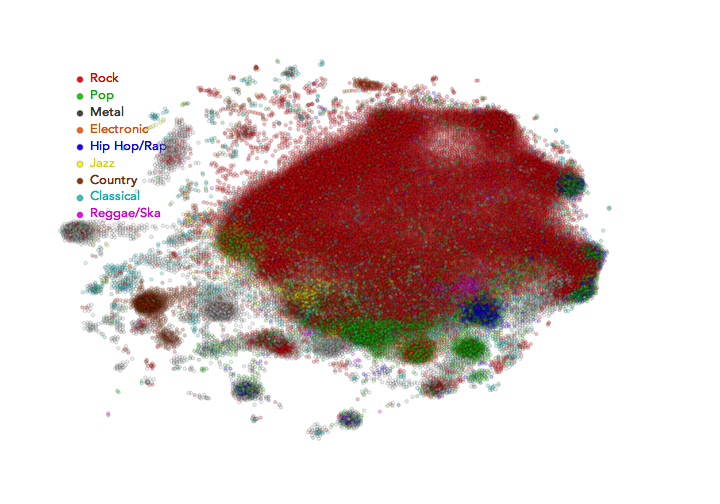
\epsfig{file=img/mystrands_08a_popular_songs_cooccurrences_unsized, width=\textwidth}
\caption{Musical associations in the data set of playlists.}
\label{fig:mystrands_bubbles}
\end{figure}
%

\subsection{Initial data set} % (fold)
\label{sub:noise_removal}

The initial data set is made of 993,825 playlists. % harvested from different Web pages. 
Playlists where any song or artist is repeated often (more than 4 times) are removed for their co-occurrence analysis would lead to the obvious outcome that a song is associated with itself or with other songs by the same artist.

In the set of remaining playlists, 5,433,413 pairs of songs appear contiguously and are not performed by the same artist. 
The most common contiguous pairs of songs are: `Dirty Little Secret' (The All-American Rejects) and `Dance, Dance' (Fall Out Boy); `Grillz' (Nelly) and  `Laffy Taffy' (D4L); `Boulevard Of Broken Dreams' (Green Day) and `Mr Brightside' (The Killers); `My Humps' (Black Eyed Peas) and `Run It!' (Chris Brown); `Caring Is Creepy' (The Shins) and `In The Waiting Line' (Zero 7); `Don't Cha' (Pussycat Dolls) and `Pon De Replay' (Rihanna).

One problem with this data set is that it contains both `good' and `bad' playlists.
People are free to publish on the Web any type of playlists and there is no implicit guarantee that the collected ones are made of songs with an affinity, as listeners can as well create and share random sets of tracks without any meaningful order.
To obtain valid musical associations, bad playlists should be removed from the data set before proceeding with the co-occurrence analysis.
% The next section describes how such playlists are identified and discarded from the data set.

%Since people are free to share any type of playlist on the Web, the data set possibly contains `good' playlists, carefully compiled with a particular purpose, and `bad' playlists, where consecutive songs do not correspond to associated songs. Hereafter, a validation method is described that measures the percentage of consecutive songs in playlists that can comprehensively be considered as associated.

% \subsubsection{Quality of the data set} % (fold)
% \label{ssub:quality_of_the_data_set}
% 
% The significance of each pair of contiguous songs is estimated with a cross-validation process.
% Let $(X,Y)$ be a pair of songs occurring contiguously in a playlist $Q$.
% This pair can either be \emph{significant} or \emph{noisy} meaning that a certain musical association can either exist or not between the two songs.
% If $X$ and $Y$ are indeed associated, then they will also co-occur often in other playlists, while if $Q$ is just a random collection of songs with no particular affinity then this would not happen.
% 
% To test the hypothesis that two songs $X$ and $Y$ are associated, the data set of playlists is partitioned in two: the playlist $Q$ where they co-occur constitutes the \emph{validation data}, while all the other playlists form the \emph{training data} (leave-one-out process).
% 
% The co-occurrence analysis process is performed on the training data to calculate the list of top associated songs with $X$; if $Y$ occurs in this list, then the hypothesis that $X$ and $Y$ are associated is confirmed.
% 
% Formally, let $s_Q: \mathcal{C}^2 \to [0,1]$ be the musical association degree \eqref{eq:final_degree} estimated analysing all the playlists but $Q$ (training data) and let $z_Q(X,Y)$ be the position of $Y$ in the ranked list of top associated tracks according to this degree:
% %
% \begin{equation*}
%  z_Q(X,Y) = \#\{Z \in \mathcal{C}\,|\,s_Q(X,Z) \geqslant s_Q(X,Y) \}\,.        
% \end{equation*}
% %
% If $z_Q(X,Y) = 1$, then $Y$ is the top associated track with $X$ according to the training set, which confirms the hypothesis that the contiguous pair of songs $(X,Y)$ in the validation data is significant.
% 
% If $z_Q(X,Y) \leqslant N$ for a given threshold $N \in \mathbb{N}^+$, then $Y$ is among the top $N$ associated tracks with $X$.
% This can also be seen as a positive validation of the hypothesis as long as $N$ is relatively small.
% If $z_Q(X,Y) > N$, the hypothesis is instead rejected.
% 
% \begin{example}
% A playlist $Q$ in the data set includes `New York, New York' (Frank Sinatra) followed by `Caravan Of Love' (The Housemartins).
% To evaluate whether an association exists between the two songs, the co-occurrence analysis process introduced in Sect.~\ref{sec:co_occurrence_analysis5} is run on all the remaining playlists, obtaining a musical association degree $s_Q$.
% According to this measure, the top associated songs with `New York, New York' (Frank Sinatra) are `The Waters Of March' (Susannah McCorkle), `Stardust' (Glenn Miller) and `New York's My Home' (Sammy Davis Jr.).
% The song `Caravan Of Love' (The Housemartins) only occurs after the first 100 positions.
% In this case, the experience of the people who compiled the remaining playlists rejects the hypothesis that the two songs are indeed associated.    
% \end{example}
% 
% The quality of the entire \emph{data set} of playlists can be measured repeating the same process for every pair of consecutive songs $(X,Y)$ in every playlist $Q$, by first calculating the top associated songs with $X$ from the training data and then verifying whether $Y$ occurs in the first $N$ positions of this list.
% 
% With a threshold of $N = 15$, the number of times the hypothesis is confirmed is 1,467,691, which corresponds to a recall of 27\%. % and is indicative of the 

% paragraph initial_data_set (end)

\subsection{Noise filtering process} % (fold)

Two hypotheses are made for filtering out bad playlists.
The first is that any playlist containing alphabetically ordered songs or artists were probably not compiled with a specific listening purpose (e.g., relaxing, jogging, partying) but as mere groups of consecutive tracks.
The second hypothesis is that neither very short nor very long playlists were created with a purpose that is coherent with the proposed interpretation of playlists.
If these playlists were discarded, then the data set would be reduced to \emph{less} playlists with a \emph{high quality}, that is, playlists which actually contain consecutive associated songs.

The noise filtering process consists in removing from the initial data set any playlist that has less than five songs, more than twenty songs, or has more than five alphabetically ordered songs or artists.
These specific values were determined after having observed the distribution of  alphabetically ordered songs and artists and the distribution of playlist lengths in the initial data set, as illustrated in Fig.~\ref{fig:alphabetical}.
%
\begin{figure}[hbtp]
\centering \setlength{\abovecaptionskip}{3pt}
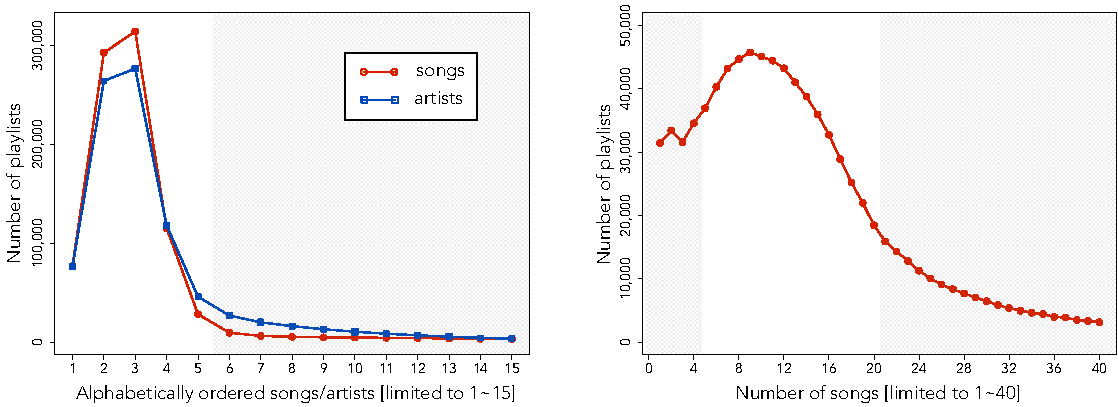
\epsfig{file=img/fig2_2, width=\textwidth}
\caption{Number of playlists with alphabetically ordered songs/artists (left) and with specific lengths (right).}
\label{fig:alphabetical}
\end{figure}

The noise filtering process reduces the data set from 993,825 to 465,438 playlists. The number of contiguous pairs of songs also decreases from 5,433,413 to 1,256,681.
% 
% \subsection{Quality assessment} % (fold)
% \label{sub:quality_of_the_initial_data}
% 
% The rationale of the noise filtering process is that working with less \emph{high quality} playlists is better than working with many \emph{low quality} playlists.
% According to the hypotheses, removing very short, very long and alphabetically ordered playlists can improve the overall quality of the data set.
% The rest of this section evaluates whether these hypotheses hold.
% 
% The first step is to provide a definition of \emph{quality} of a set of playlists. 
% The quality of a set of playlists is the percentage of pairs of songs that occur consecutively in one playlist and, according to the remaining playlists, are musically associated.
% 
% Formally, let $(X,Y)$ be two consecutive songs occurring in a playlist $Q$ and let $s_Q(X,Y)$ be the musical association degree \eqref{eq:final_degree} calculated from the co-occurrences of $X$ and $Y$ in the remaining playlists.
% The more the other playlists where $X$ and $Y$ appear together and the closer their co-occurrences, the higher the value of $s_Q(X,Y)$.
% 
% Let $z_Q(X,Y)$ be the number of songs that are musically associated with $X$ at least as much as $Y$: %, calculated according to all the remaining playlists:
% %
% \begin{equation*}
%  z_Q(X,Y) = \#\{Z \in \mathcal{C}\,|\,s_Q(X,Z) \geqslant s_Q(X,Y) \}\,.        
% \end{equation*}
% %
% If $z_Q(X,Y) \leqslant N$ for a relatively small threshold $N \in \mathbb{N}^+$, then $Y$ is one of the top associated tracks with $X$ according to the remaining playlists. In this case, the analysis of the data set confirms that the contiguous pair $(X,Y)$ corresponds to two associated songs. 
% 
% If $z_Q(X,Y) > N$, then the pair $(X,Y)$ corresponds instead to \emph{noise}: two songs that by chance occur together in one playlist but whose association is not endorsed by the rest of the data set.
% 
% Given these definitions, the quality of the initial data set can be compared with the quality of the filtered data set to test the effectiveness of the noise filtering process. The threshold is fixed to the value of $N = 15$.
% 
% The initial data set contains 5,433,413 pairs of consecutive songs $(X,Y)$; the number of times when $Y$ is confirmed as one of the top $N$ associated tracks with $X$ is 1,467,691.
% 
% Discarding playlists with more than five alphabetically ordered elements reduces these values respectively to 2,710,843 and 765,623. The ratio of these values is 28.2\%, which is 4.5\% higher than the ratio in the initial data set (27\%). This supports the first hypothesis.
% 
% Discarding playlists with less than five or more than twenty songs further reduces the number of pairs of contiguous songs to 1,256,681 and the number of times each pair is confirmed as one of the top $N = 15$ associated to 386,164. The ratio in this case is 30.7\% which is 8.8\% higher than in the initial data set. This supports the second hypothesis.
% %
% 

\section{Tuning parameters} % (fold)
\label{sub:tuning_parameters}

The next step before applying the co-occurrence analysis process to the filtered set of playlists is to decide the values of different parameters introduced in Sect.~\ref{sec:co_occurrence_analysis5}.
The parameters are $\delta$, $\alpha_J$ and $\gamma$, which occur in the functions \eqref{eq:item_association} and \eqref{eq:final_degree}.
These parameters determine how much the distance and the order of songs in playlists influence their association.

\subsection{Tuning the distance parameters} % (fold)
\label{par:considering_separated_songs_}
% [NOTE: These are the results where I also exclude songs that occur in less than 5 playlists, I'm calculating them anew without this filter].

The maximum distance parameter is set to $\delta = 3$, which stands as a compromise between contiguous and distant co-occurrences.
This means that two songs that appear in the same playlist separated by less than three songs are considered as associated, otherwise the association does not subsist.

%The data set includes 1,244,555 pairs of songs that co-occur in a playlist within a distance of $\delta = 3$.

The distance parameters $\alpha_1, \alpha_2, \alpha_3 \in [0,1]$ determine the degree in which closer co-occurrences are more relevant than distant ones.
These parameters are set to $\alpha_1 = 0.6, \alpha_2 = 0.3, \alpha_3 = 0.1$ to gradually assign higher importance to closer co-occurrences.

%The decision about these particular values was taken with a process similar to the one presented in the previous section, comparing for each pair of consecutive songs $(X,Y)$ in the data set the number of times that $Y$ would appear in the list of top $N$ associated tracks with $X$ under different values of $\alpha_1$, $\alpha_2$ and $\alpha_3$.

%The entire data set contains 1,244,555 pairs of songs $(X,Y)$ occurring within a distance of $\delta = 3$ and, with the parameters set to  $\alpha_1 = 0.6, \alpha_2 = 0.3, \alpha_3 = 0.1$, the number of times that $Y$ is found in the list of top $N = 15$ associated ones with $X$ is 387,313. %, corresponding to a ratio of 30.8\%.

%On the contrary, considering only adjacent co-occurrences (that is, setting the parameters to $\alpha_1 = 1, \alpha_2 = \alpha_3 = 0$) would result in a lower number of 386,184 pairs. % of consecutive songs identified as associated, with a ratio of 30.7\%.
%
%Similarly, assigning the same importance to co-occurrences at different distances ($\alpha_1 = \alpha_2 = \alpha_3 = \frac{1}{3}$) would result in only 357,232 pairs of associated songs. %, with a smaller ratio of 28.4\%.

% paragraph considering_separated_songs_ (end)

% $\frac{357,232}{15*1,224,555} = 1.94\%$, while the case of $\beta = 0.5$ makes me predict the right successor in 387,313 cases with N = 15, which gives a precision of $\frac{387,313}{15*1,224,555} = 2.11\%$, which is (a 2.4\%) higher than before. So considering different distances makes sense.

\subsection{Tuning the order parameter} % (fold)
\label{par:considering_different_orderings_}

%The more two songs $(X,Y)$ occur in the same order, the more they go well together in that order.
The parameter $\gamma \in [0,0.5]$ determines the degree in which inverse co-occurrences ($X$ \emph{after} $Y$) also contribute to determine their associations.
%
In this case, this parameter is set to $\gamma = 0.2$: direct co-occurrences (where $X$ occurs \emph{before} $Y$) are identified as more relevant to determine the association between $X$ and $Y$ than inverse co-occurrences.

%As for the distance parameters, this value was decided after comparing different possible scenarios. % and selecting the one which returned the highest ratio of consecutive songs identified as associated.
%
%With the parameter set to $\gamma = 0$, the number of consecutive pairs of songs $(X,Y)$ for which $Y$ results in the list of top $N = 15$ associated tracks with $X$ is 387,313.

%On the contrary, assigning the same importance to direct and inverse co-occurrences ($\gamma = 0.5$) would result in a smaller value of 347,362.
%Assigning a slighter large influence to direct than to inverse co-occurrences ($\gamma = 0.25$) would also return a smaller value (372,995).

Setting the parameter to $\gamma = 0.2$ expresses the fact that the order in which two songs occur in playlists has an effect on the measure of their association. 
This value was decided observing that many playlists in the data set are \emph{asymmetric} by nature: songs sound well together in one direction but not necessarily in the other one. 
This can be explained by the fact that several authors, especially disc jockeys, compile playlists where the \emph{end} of each song mixes with the \emph{beginning} of the next one.
In these cases, the order should be accounted for when measuring associations.



% \subsection{Distance and order of co-occurrences} % (fold)
% \label{sub:tuning_parameters}
% 
% The noise filtering process has identified, within the initial data set of playlist, a subset of `good' playlists on which to apply the co-occurrence analysis process described in Sect.~\ref{sec:co_occurrence_analysis5} to measure musical associations.
% 
% Before running the analysis, the values of the parameters $\delta$, $\alpha_J$ and $\gamma$ that occur in the functions \eqref{eq:item_association} and \eqref{eq:final_degree} have to be decided, indicating how much the distance and the order of songs in playlists influence their association.
% 
% \subsubsection{Tuning the distance parameters} % (fold)
% \label{par:considering_separated_songs_}
% 
% The maximum distance is set to $\delta = 3$, a compromise between contiguous and distant co-occurrences. Songs that occur in the same playlist separated by more than three songs are not considered as associated.
% 
% In order to gradually assign more importance to closer co-occurrences, the distance parameters $\alpha_1, \alpha_2, \alpha_3 \in [0,1]$ are set to the values $\alpha_1 = 0.6, \alpha_2 = 0.3, \alpha_3 = 0.1$.
% 
% \subsubsection{Tuning the order parameter} % (fold)
% \label{par:considering_different_orderings_}
% 
% The order parameter $\gamma \in [0,0.5]$ determines the degree in which inverse co-occurrences ($X$ \emph{after} $Y$) also contribute to determine their associations.
% This parameter is set to $\gamma = 0.2$ to assign only a small importance to inverse co-occurrences.
% The motivation is that playlists are often not symmetric.
% Songs can be ordered with a specific purpose that does not hold if reversed, for instance when the end of a song mixes well with the beginning of the next one.
% 



\section{The resulting associations} % (fold)
\label{sub:the_smoothness_degrees_we_obtain}

%Filtering out alphabetically ordered playlists and playlists that are too short or long improves the quality of the data set with respect to the musical associations. Considering separated songs with decreasing weights according to the distance is also important, while considering co-occurrences in both orders does not seem relevant.

Having filtered noise from the initial data set of 993,825 playlists and having applied the co-occurrence analysis technique with the parameters set to:
\begin{itemize}
 \item maximum distance between songs: $\delta = 3$,
 \item degrees in which distance influences the strength of the association: $\alpha_1 = 0.6, \alpha_2 = 0.3, \alpha_3 = 0.1$,
 \item degree in which popularity bias is punished:  $\beta = 0.8$,
 \item degree in which order influences %the strength of 
 the association: $\gamma = 0.2$,
 \item degrees in which different types of co-occurrences influence the strength of the association: $\phi_1 = 0.6, \phi_2 = 0.3, \phi_3 = 0.1$,
\end{itemize}
the association degrees $s(X,Y)$ defined in Sect.~\ref{sec:co_occurrence_analysis5} are finally calculated.

Associations between songs by the same artist are excluded for their obviousness, as well as songs by `virtual' artists (such as `Various Artists' or `Soundtrack') and songs appearing in less than 5 playlists, for their minimal statistical significance.
This threshold was fixed observing how the popularity of songs distributes in the data set of playlists (Fig.~\ref{fig:lengths}).
%
\begin{figure}[hbtp]
\centering \setlength{\abovecaptionskip}{3pt}
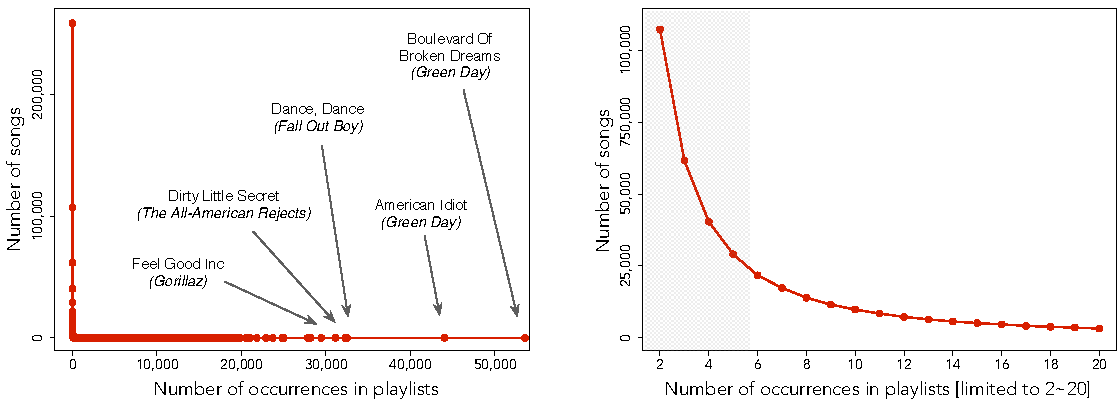
\epsfig{file=img/fig2_3, width=\textwidth}
\caption{Occurrences per songs in retrieved playlists.}
\label{fig:lengths}
\end{figure}

Eventually, a musical association degree $s(X,Y)$ was estimated for as many as 46,217,300 % this includes artist-to-artist
distinct pairs of 415,498 songs by 47,148 distinct artists.

%Two examples of musical associations found for a given song and artists are presented hereafter. %; other examples are reported with their evaluation in Chap.~\ref{cha:evaluation}.

% \begin{example}\label{ex:flymetothemoon}
% The song `Fly Me To The Moon' (Astrud Gilberto) occurs in 364 playlists. % compiled by MusicStrands members.
% The analysis finds out that 182 songs appear in playlists with `Fly Me To The Moon', that 52 songs appear in playlists with other songs by Astrud Gilberto, and that 194 songs are from artists appearing in playlists with songs by Astrud Gilberto.
% The co-occurrence analysis allows to rank all these songs according to how much they are associated with `Fly Me To The Moon', uncovering the following songs as the top associated: `Come Fly With Me' (Frank Sinatra), `L-O-V-E' (Nat King Cole), `What A Wonderful World' (Louis Armstrong), `I've Got The World On A String' (Frank Sinatra), `Ain't That A Kick In The Head' (Dean Martin), `Beyond The Sea' (Bobby Darin), `At Last' (Etta James) and `Kissing A Fool' (Michael Bubl\'{e}).
% \end{example}
% 
% \begin{example}
% Songs from the band Panic!\;At The Disco occur in 29,052 playlists.
% The analysis finds out that songs by 5,170 distinct artists appear in playlists with any song by Panic!\;At The Disco and rank their artists according to how much they are musically associated with Panic!\;At The Disco.
% The following artists are uncovered as the most associated: October Fall, Pilot Speed, My American Heart, Nightmare Of You, The Presets, The Pink Spiders and Junior Boys.
% % NOTE: ADD MySpace links to all these groups!!
% \end{example}
% 

\subsection{Evaluating song associations} % (fold)
\label{sub:evaluating_song_association}

Given a song $X$ in the data set, the songs $Y$ with the highest association degree $s(X,Y)$ are the songs that go best in a sequence after $X$ according to the human experience recorded in playlists.
The following is an example of list of top associated tracks.

\begin{example}\label{ex:newyork}
The song `New York, New York' (Frank Sinatra) occurs in 219 playlists.
The analysis finds that 173 distinct songs appear in playlists with `New York, New York', that 6,458 songs appear in playlists with other songs by Frank Sinatra, and that 26,402 songs are from artists appearing in playlists with songs by Frank Sinatra.
The co-occurrence analysis allows to rank all these songs according to how much they are associated with `New York, New York', uncovering the following songs as the top associated ones:  `The Waters Of March' (Susannah McCorkle), `Stardust' (Glenn Miller), `New York's My Home' (Sammy Davis Jr.), `Manhattan Avenue' (Nellie McKay), `Mississippi Goddam' (Nina Simone), `Something Beautiful' (Robbie Williams).
\end{example}

The example highlights some common properties of the lists of top associated songs.
The first characteristic is that the top songs are not particularly famous, yet share a strong affinity with the seed track.
 `The Waters Of March' (Susannah McCorkle), for instance, is strongly connected with `New York, New York' (Frank Sinatra) since they were both composed in the Seventies and performed as musical standards by various singers.
The reason why uncommon songs appear higher in the list is the high value of the popularity bias parameter $\beta = 0.8$ which punishes songs that occur very often in the set of playlists.

Another positive characteristic of the list is diversity: all the songs are performed by different artists and belong to multiple genres and periods; `Something Beautiful' (Robbie Williams), for instance, was published in 2003.


\subsection{Evaluating artist association} % (fold)

As well as lists of top associated tracks, the co-occurrence analysis can produce lists of top associated artists.
Given an artist $a(X)$ in the data set, the artists whose songs have in average the highest association degree with the songs of $a(X)$ are the top associated artists with $a(X)$.

Working at the level of artists is not as specific as working at the level of songs: two songs can go well together for acoustic reasons (same timbre, rhythm, lyrics) while a correlation between two artists is more abstract, implying some sort of social or cultural relationships (e.g., two artists are contemporary, play the same instrument, have collaborated, belong to the same genre).
An example of list of top associated artists is reported hereafter.

\begin{example}
Themes written by the soundtrack composer John Williams appear in 2,367 playlists.
The analysis finds out that songs by 866 distinct artists appear in playlists with any track by John Williams. These artists are ranked according to how much they are musically associated with John Williams;
the following artists are uncovered as the most associated: Itzhak Perlman, Christopher Young, Arthur Fiedler, London Symphony Orchestra, John Debney, Danny Elfman, John Carpenter, John Barry.
% NOTE: ADD MySpace links to all these groups!!
\end{example}

Similarly to Example~\ref{ex:newyork}, an interesting property of this list is that uncommon but strongly associated items appear first, followed by more popular ones.
Itzhak Perlman, for instance, is not a soundtrack composer but a violinist who played first violin in `Schindler's List' soundtrack, composed by John Williams.
Arthur Fiedler also shares a strong affinity with John Williams, who took his place as the conductor of the Boston Pops orchestra in 1979 after Fiedler's death.
John Debney, Danny Elfman and John Barry are award-winning movie composers contemporary to John Williams.

\subsection{Comparisons with other music similarity measures} % (fold)
\label{sub:comparisons_with_music_similarity_measures}

%The lists of top associated songs and artists obtained point out which items are more indicate to be played in sequence.
For the purpose of evaluation, some lists of top associated songs and artists are hereafter contrasted with equivalent lists calculated with distinct sources of musical knowledge obtained from different Web sites.
The Web sources used for the comparison are: Yahoo! Music, Last.fm and Audiobaba for associated songs and All Music Guide, Yahoo! Music, Last.fm, MusicStrands and MusicSeer for associated artists.
The technique presented in this chapter does not exactly look for `similar' songs, but for songs that go well together in sequence.
Nevertheless, comparing its assessments with those offered by other techniques can reveal interesting peculiarities.

Yahoo! Music makes available for each song and artist in its catalogue a list of similar tracks and artists ``generated from end user feedback'' \cite{Baumann04}.
Last.fm offers for each song a Web page listing what people who listened to that song also listened to.
Audiobaba uses a content-based approach: for each song, a list of tracks that are acoustically similar is returned.

For associations among artists, All Music Guide includes handcrafted contributions written by expert editors and is considered as the `bible' of music reviews, the ground truth for music classification research \cite{Pachet00b,Hu07,Magno08,Sordo08}.
MusicStrands derives associations from the same data set of playlists employed in this dissertation, but applying a different technique based on ``bags of associations'' \cite{Shur06}.
MusicSeer follows two different approaches: one is based on a survey to collect subjective judgements about artist similarity, the other one on playlist co-occurrences. 
The MusicSeer survey includes associations for about 413 artists \cite{Logan03}, while the playlist-based approach reports associations between 60,931 artists from the analysis of 29,164 playlists retrieved from Art Of The Mix \cite{Ellis03}.

Tables~\ref{table:samplerelevance}, \ref{table:samplerelevance2} and~\ref{table:samplerelevance3} report the most associated tracks for the songs `New York, New York' (Frank Sinatra), `Whenever, Wherever' (Shakira) and `Smoke On The Water' (Deep Purple).
Tables~\ref{table:samplerelevance4}, \ref{table:samplerelevance5}, \ref{table:samplerelevance6} and \ref{table:samplerelevance7} compare the top artists delivered for John Williams, Frank Sinatra, Abba and Destiny's Child. 

\begin{table}[bthp]\centering
\setlength{\extrarowheight}{3pt}
\setlength{\abovecaptionskip}{3pt}
\setlength{\belowcaptionskip}{3pt}
\setlength{\intextsep}{0pt}
\caption{Top associated songs for `New York, New York' (Frank Sinatra).}\label{table:samplerelevance}
{\fontsize{8}{10}\selectfont
\begin{tabular}{|c|p{0.8\textwidth}|}
 \hline 
 \multirow{3}{*}{Poolcasting} &
 `The Waters Of March' (Susannah McCorkle), `Stardust' (Glenn Miller), `New York's My Home' (Sammy Davis Jr.), `Manhattan Avenue' (Nellie McKay), `Mississippi Goddam' (Nina Simone), `Something Beautiful' (Robbie Williams) \vspace{2pt} \\
 \hline
 \multirow{3}{*}{Yahoo!} &
 `Piano Man' (Billy Joel), `That's Amore'	(Dean Martin), `At Last' (Etta James), `Mrs. Robinson'	(Simon \& Garfunkel), `The Boxer' (Simon \& Garfunkel), `Bridge Over Troubled Water' (Simon \& Garfunkel) \vspace{2pt} \\
 \hline
 \multirow{3}{*}{Last.fm} &
 `Strangers In The Night' (Frank Sinatra), `Fly Me To The Moon'	(Frank Sinatra), `What A Wonderful World' (Louis Armstrong), `Walkin' My Baby Back Home'	(Nat King Cole), `Try To Remember' (Bobby Darin), `Beyond The Sea' (Bobby Darin) \vspace{2pt} \\
 \hline
 \multirow{3}{*}{Audiobaba} &
 `Woman, Woman' (Gary Puckett), `Spirit In The Night'	(Bruce Springsteen), `You Make Me Feel So Young' (Frank Sinatra), `Mud On The Tires'	(Brad Paisley), `Lucky To Be Here' (Montgomery Gentry), `6 AM' (Random Access) \vspace{2pt} \\
 \hline
 \noalign{\bigskip}
\end{tabular}}
\end{table}
%{\setlength{\intextsep}{0pt}
\begin{table}[bthp]\centering
\setlength{\extrarowheight}{3pt}
\setlength{\abovecaptionskip}{3pt}
\setlength{\belowcaptionskip}{3pt}
\caption{Top associated songs for `Whenever, Wherever' (Shakira).}\label{table:samplerelevance2}
{\fontsize{8}{10}\selectfont\begin{tabular}{|c|p{0.8\textwidth}|}
 \hline
 \multirow{3}{*}{Poolcasting} &
 `You Spin Me Round' (Thal\'{\i}a), `Crazy In Love' (Beyonc\'{e} \& Jay-Z), `Grazing In the Grass' (Raven-Symon\'{e}), `Si Ya Se Acab\'{o}' (Jennifer Lopez), `Freakout' (B*Witched), `Perros' (Paulina Rubio) \vspace{2pt} \\ 
 \hline
 \multirow{3}{*}{Yahoo!} &
 `Baby One More Time'	(Britney Spears), `Irresistible'	(Jessica Simpson), `If You Had My Love' (Jennifer Lopez), `Candy'	(Mandy Moore), `Bye Bye Bye'	('N Sync), `Genie In A Bottle' (Christina Aguilera) \vspace{2pt} \\
 \hline
 \multirow{3}{*}{Last.fm} &
 `Underneath Your Clothes'	(Shakira), `Objection (Tango)'	(Shakira), `Radar' (Britney Spears), `Keeps Gettin' Better'	(Christina Aguilera), `Beautiful Liar'	(Beyonc\'{e} feat. Shakira), `Waiting for Tonight' (Jennifer Lopez) \vspace{2pt} \\
 \hline
 \multirow{3}{*}{Audiobaba} &
 `Too Bad'	(Bad Company), `Sunday Girl'	(Erasure), `Life In The Fast Lane' (Eagles), `These Dreams Of You Are So Much Sweeter Than The Truth'	(The Sharp Things), `Powerful Thing'	(Trisha Yearwood), `Migration' (Jimmy Buffett) \vspace{2pt} \\
 \hline
\end{tabular}}
\end{table}
%}
%{\setlength{\intextsep}{0pt}
\begin{table}[bthp]\centering
\setlength{\extrarowheight}{3pt}
\setlength{\abovecaptionskip}{3pt}
\setlength{\belowcaptionskip}{3pt}
\caption{Top associated songs for `Smoke On The Water' (Deep Purple).}\label{table:samplerelevance3}
{\fontsize{8}{10}\selectfont\begin{tabular}{|c|p{0.8\textwidth}|}
 \hline
 \multirow{3}{*}{Poolcasting} &
 `Silver Machine' (Hawkwind), `The Joker' (Steve Miller Tribute Band), `Dream Evil' (Dio), `Rock N' Roll Hoochie Koo' (Johnny Winter), `South Saturn Delta' (Jimi Hendrix), `Nottingham Lace' (Buckethead) \vspace{2pt} \\ 
 \hline
 \multirow{3}{*}{Yahoo!} &
 `Melissa'	(The Allman Brothers Band), `Surrender'	(Cheap Trick), `Sweet Talkin' Woman' (Electric Light Orchestra), `Somebody To Love'	(Jefferson Airplane), `White Rabbit'	(Jefferson Airplane), `Maggie May' (Maggie May) \vspace{2pt} \\
 \hline
 \multirow{3}{*}{Last.fm} &
 `Highway Star'	(Deep Purple), `Child in Time'	(Deep Purple), `Stairway to Heaven' (Led Zeppelin), `Paranoid'	(Black Sabbath), `Whole Lotta Love'	(Led Zeppelin), `Black Dog' (Led Zeppelin) \vspace{2pt} \\
 \hline
 \multirow{3}{*}{Audiobaba} &
 `Double E'	(Neil Young), `This Can't Be Love'	(Freeborn), `The Lady' (TheHookUp), `Elegant People'	(Jaco Pastorius Big Band), `Last Chance'	(Ear Candy), `Diggers Of Ditches Everywhere' (These Arms Are Snakes) \vspace{2pt} \\
 \hline
\end{tabular}}
\end{table}
%}
%{\setlength{\intextsep}{0pt}
\begin{table}[bhtp]\centering
\setlength{\extrarowheight}{3pt}
\setlength{\abovecaptionskip}{3pt}
\setlength{\belowcaptionskip}{3pt}
\setlength{\intextsep}{0pt}
\caption{Top associated artists for John Williams.}\label{table:samplerelevance4}
{\fontsize{8}{10}\selectfont
\begin{tabular}{|c|p{0.8\textwidth}|}
 \hline 
 \multirow{2}{*}{Poolcasting} &
 Itzhak Perlman, Christopher Young, Arthur Fiedler, London Symphony Orchestra, John Debney, Danny Elfman, John Carpenter, John Barry \vspace{2pt} \\
 \hline
 \multirow{2}{*}{MusicStrands} &
 Danny Elfman, Vangelis, Hollywood Studio Orchestra, Erich Kunzel, Green Day, Gorillaz, Weird Al Yankovic, John Barry, Queen, Eminem \vspace{2pt} \\
 \hline
 AllMusic &
 John Barry, Jerry Goldsmith, Elmer Bernstein, Howard Shore, Erich Korngold \vspace{2pt} \\
 \hline
 \multirow{2}{*}{Yahoo!} &
 Franz Joseph Haydn, James Newton Howard, Michael Kamen, National Philarmonic Orchestra, Alan Silvestri, Jerry Goldsmith, John Barry \vspace{2pt} \\
 \hline
 \multirow{2}{*}{Last.fm} &
 Jerry Goldsmith, James Horner, Patrick Doyle, Alan Silvestri, James Newton Howard, Howard Shore, Hans Zimmer, Nicholas Hooper, Danny Elfman \vspace{2pt} \\
 \hline
 \noalign{\bigskip}
\end{tabular}}
\end{table}
%}
%{\setlength{\intextsep}{0pt}
\begin{table}[bhtp]\centering
\setlength{\extrarowheight}{3pt}
\setlength{\abovecaptionskip}{3pt}
\setlength{\belowcaptionskip}{3pt}
\setlength{\intextsep}{0pt}
\caption{Top associated artists for Frank Sinatra.}\label{table:samplerelevance5}
{\fontsize{8}{10}\selectfont
\begin{tabular}{|c|p{0.8\textwidth}|}
 \hline 
 \multirow{2}{*}{Poolcasting} &
 Dean Martin, Sammy Davis Jr., Judy Garland, Bing Crosby, The California Raisins, Tony Bennett, Louis Prima, Rosemary Clooney, Nat King Cole \vspace{2pt} \\
 \hline
 \multirow{2}{*}{MusicStrands} &
 Dean Martin, Billie Holiday, Nat King Cole, Perry Como, Ella Fitzgerald, Andy Williams, Tony Bennett, Etta James, Bing Crosby, Diana Krall \vspace{2pt} \\
 \hline
 \multirow{2}{*}{AllMusic} &
 Dean Martin, Vic Damone, Dick Haymes, Sarah Vaughan, Nat King Cole, Dinah Washington, Mel Torm\'{e}, Ella Fitzgerald, Tony Bennett, Jo Stafford \vspace{2pt} \\
 \hline
 \multirow{2}{*}{Yahoo!} &
 Dean Martin, Tony Bennett, Nat King Cole, Ray Charles, The Beach Boys, Simon \& Garfunkel, Elvis Presley, The Beatles, Norah Jones, Norah Jones  \vspace{2pt} \\
 \hline
 \multirow{2}{*}{Last.fm} &
 Dean Martin, Sammy Davis, Jr., Frank Sinatra \& Tommy Dorsey, Tony Bennett, Nat King Cole, Bobby Darin, Ella Fitzgerald, Mel Torm\'{e} \vspace{2pt} \\
 \hline
 \multirow{2}{*}{MS Survey} &
 Eric Clapton, Billy Joel, Elton John, Elvis Costello, Elvis Presley, Van Morrison, John Lennon, Bob Dylan, Nine Days, Ozzy Osbourne \vspace{2pt} \\
 \hline
 \multirow{2}{*}{MS Playlists} &
 Elvis Presley, Elton John, John Denver, Abba, Whiskeytown, Beatles, Billy Joel, Bob Marley, Eric Clapton, Everly Brothers \vspace{2pt} \\
 \hline
 \noalign{\bigskip}
\end{tabular}}
\end{table}
%}
\begin{table}[bhtp]\centering
\setlength{\extrarowheight}{3pt}
\setlength{\abovecaptionskip}{3pt}
\setlength{\belowcaptionskip}{3pt}
\setlength{\intextsep}{0pt}
\caption{Top associated artists for Abba.}\label{table:samplerelevance6}
{\fontsize{8}{10}\selectfont
\begin{tabular}{|c|p{0.8\textwidth}|}
 \hline 
 \multirow{2}{*}{Poolcasting} &
 Agnetha F\"{a}ltskog, A-Teens, Chic, Gloria Gaynor, The 5th Dimension, Andy Gibb, Olivia Newton-John, Rose Royce, KC \& The Sunshine Band, Bee Gees \vspace{2pt} \\
 \hline
 \multirow{2}{*}{MusicStrands} &
 Donna Summer, Madonna, Gloria Gaynor, Cyndi Lauper, Blondie, Kool \& The Gang, Elton John, The B-52s, Michael Jackson, Diana Ross \vspace{2pt} \\
 \hline
 \multirow{2}{*}{AllMusic} &
 Ambsoris, Olivia Newton-John, The Carpenters, Captain \& Tennille, Bucks Fizz, Fletwood Mac, Andy Gibb, Lindsey Buckingham, The Cowsills \vspace{2pt} \\
 \hline
 \multirow{2}{*}{Yahoo!} &
 Bee Gees, The Carpenters, Elvis Presley, The Beatles, Foreigner, Whitney Houston, Bon Jovi, Madonna, Barry Manilow, Michael Jackson \vspace{2pt} \\
 \hline
 \multirow{2}{*}{Last.fm} &
 Agnetha F\"{a}ltskog, Frida, Boney M., Bee Gees, Olivia Newton-John, Baccara, Cher, Bucks Fizz, Donna Summer, Army of Lovers, Alcazar \vspace{2pt} \\
 \hline
 \multirow{2}{*}{MS Survey} &
 Ace of Base, Bee Gees, Blondie, Spice Girls, Olivia Newton-John, Beach Boys, Roxette, Cyndi Lauper, Backstreet Boys, Donna Summer \vspace{2pt} \\
 \hline
 \multirow{2}{*}{MS Playlists} &
 Bee Gees, Blondie, Cyndi Lauper, Queen, Cat Stevens, Cher, Beach Boys, Donna Summer, Olivia Newton-John, Phil Collins \vspace{2pt} \\
 \hline
 \noalign{\bigskip}
\end{tabular}}
\end{table}
%
%{\setlength{\intextsep}{0pt}
\begin{table}[bhtp]\centering
\setlength{\extrarowheight}{3pt}
\setlength{\abovecaptionskip}{3pt}
\setlength{\belowcaptionskip}{3pt}
\setlength{\intextsep}{0pt}
\caption{Top associated artists for Destiny's Child.}\label{table:samplerelevance7}
{\fontsize{8}{10}\selectfont
\begin{tabular}{|c|p{0.8\textwidth}|}
 \hline 
 \multirow{2}{*}{Poolcasting} &
 Kelly Rowland, City High, Ciara, Fantasia, Christina Milian, Beyonc\'{e}, Ashanti, Girls Aloud, 3LW, Dru Hill \vspace{2pt} \\
 \hline
 \multirow{2}{*}{MusicStrands} &
 Ciara, Pussycat Dolls, Usher, Beyonc\'{e}, Nelly, 50 Cent, Mariah Carey, Chris Brown, Gwen Stefani, Eminem \vspace{2pt} \\
 \hline
 \multirow{2}{*}{AllMusic} &
 Toni Braxton, Mariah Carey, Jennifer Lopez, Aaliyah, Xscape, Ginuwine, Deborah Cox, Kelly Price, Faith Evans, Brandy, Usher, Mya \vspace{2pt} \\
 \hline
 \multirow{2}{*}{Yahoo!} &
 Faith Evans, Cruel Story Of Youth, Nich Lachey, Jamie Foxx, Jessica Simpson, Ciara, Jagged Edge, Lil' Kim, Ryan Cabrera, Janet Jackson \vspace{2pt} \\
 \hline
 \multirow{2}{*}{Last.fm} &
 Beyonc\'{e}, Kelly Rowland, Michelle Williams, LeToya, Solange, Ashanti, Ciara, Brandy, Mariah Carey, Monica, Aaliyah, TLC, Mya \vspace{2pt} \\
 \hline
 \noalign{\bigskip}
\end{tabular}}
\end{table}
%}
%

The analysis of these lists of top associated songs does not reveal a great diversity among different musical sources, although some peculiarities can be observed.
As noted previously, co-occurrence analysis of playlists can identify songs that are associated but not overly popular, something that does not happen with every other technique.
Yahoo! Music, for instance, returns the famous hit `Baby One More Time' (Britney Spears) as the top associated song for `Whenever, Wherever' (Shakira). For this song, `You Spin Me Round' (Thal\'{\i}a) is possibly a better match since both songs were released in 2001 and performed by Latin American singers (see Table~\ref{table:samplerelevance2}).
Another observation is that Last.fm and Yahoo! Music have limited diversity in the results: Last.fm returns two tracks by Frank Sinatra as the top associated for `New York, New York' (see Table~\ref{table:samplerelevance}) while Yahoo! Music repeats songs by the same artists  (Simon \& Garfunkel in Table~\ref{table:samplerelevance} and Jefferson Airplane in Table~\ref{table:samplerelevance3}).

The analysis of top associated artists also reveals particular behaviours for the different methods.
First, almost every source of knowledge yields Dean Martin as the top associated artist with Frank Sinatra (see Table~\ref{table:samplerelevance5}), marking a clear affinity between the two.
Next, the playlist-based approach introduced in this chapter returns first artists that are not very popular but strongly associated.

An example is provided by Table~\ref{table:samplerelevance6} where Agnetha F\"{a}ltskog shows up as the top associated artist for Abba according to the co-occurrence analysis of playlists. 
Agnetha F\"{a}ltskog is not a very famous solo artist but she is indeed popularly known as the lead singer of Abba.
Similarly, Table~\ref{table:samplerelevance7} shows Kelly Rowland (one of the members of Destiny's Child) as one of the top associated artist with Destiny's Child.

This behaviour is possibly the most distinct advantage of the playlist-based method: to be able to spot out items that share a strong social affinity. % better than items that just happen to be very popular.
This result is obtained from the automatic analysis of playlists, without human intervention.
All Music Guide, on the other hand, requires man-hours of dedicated expert work to obtain results that are almost equivalent in terms of affinity and sometimes worse in terms of diversity.

% This effect is mainly produced by the popularity bias parameter set to $\beta = 0.8$ that pushes down in the list artists that are over-popular in the set of analysed playlists.
% 
% 
% %\paragraph{Observations.} % (fold)
% %\label{par:observations_}
% 
% The proposed technique tends to return top associated songs that are generally not as popular as those returned by other methods.
% Susannah McCorkle, for instance, is probably not as famous as Billy Joel or Frank Sinatra (see Table~\ref{table:samplerelevance}), still her version of `The Waters of March'\,---a bossa nova standard\,---\,has a strong musical association with `New York, New York'.
% Likewise, Thal\'{\i}a's version of `You Spin Me Round' is not as famous as `Baby One More Time' (Britney Spears) (see Table~\ref{table:samplerelevance2}) but is possibly more musically associated with `Whenever, Wherever' (Shakira), since both songs were performed by Latin American singers and released in 2001.
% 
% In general, the proposed technique shows first songs that are strongly associated although not very popular, followed by songs that are more popular, such as `Crazy In Love' (Beyonc\'{e} \& Jay-Z) in Table~\ref{table:samplerelevance2}.
% This behaviour is the direct consequence of the popularity bias parameter set to $\beta = 0.8$; with a lower value, over-popular songs would show up earlier in the list.
% 
% Another observation is how most of the top associated tracks according to playlist co-occurrences `sound similar', although no acoustic-based analysis has been performed.
% Moreover, in all three examples, Last.fm returns tracks by the same artists as the most associated, while the proposed technique explicitly avoids this kind of outcome for its obviousness.
% Diversity among the results is also important; as a matter of fact all the top associated songs returned are performed by different artists while Yahoo! Music tends instead to repeat the same artists in the list of similar songs (Simon \& Garfunkel in Table~\ref{table:samplerelevance} and Jefferson Airplane in Table~\ref{table:samplerelevance3}).
% 
% % paragraph observations_ (end)
% 
% 
% \subsection{Evaluating artist association} % (fold)
% 
% The artist-to-artist association function \eqref{eq:artist_to_artist} identifies associated artists whose songs go well together in sequence.
% 
% Lists of top associated artists calculated with the function  \eqref{eq:artist_to_artist} are compared hereafter with the lists of most similar artists retrieved from the following music sources: All Music Guide, Yahoo! Music, Last.fm, MusicStrands and MusicSeer.
% 
% 
% 
% 
% %\paragraph{Observations.} % (fold)
% %\label{par:observations2}
% 
% As for song-to-song associations, the proposed technique is able to spot out, as top associated, artists that are not extremely popular but share a strong relationship with the seed artist.
% Agnetha F\"{a}ltskog, for instance, is not a very famous solo artist but is popularly known as the lead singer of Abba (see Table~\ref{table:samplerelevance4}); Itzkah Perlman played first violin in `Schindler's List' soundtrack, directed by John Williams (see Table~\ref{table:samplerelevance5}); Kelly Rowland was a member of the band Destiny's Child (see Table~\ref{table:samplerelevance6}).
% %
% This effect is mainly produced by the popularity bias parameter set to $\beta = 0.8$ that pushes down in the list artists that are over-popular in the set of analysed playlists.
% 
% Another interesting observation is how, in the case of Frank Sinatra, most techniques return Dean Martin as the top associated artist (see Table~\ref{table:samplerelevance7}), although based on different types of knowledge.
% 
% The proposed technique also behave well when compared to All Music Guide, which is often considered as a base referrer for its associations are compiled by hands by a group of experts.
% The main advantage of the proposed technique is that it is autonomous and scalable, while All Music Guide requires many man-hours to obtain similar results.
% 
% % after Fiedler's death in 1979, the conductorship of the Boston Pops was taken over by John Williams.
% 

% paragraph observations2 (end)

% section the_experiments2 (end)

\section{Summary} % (fold)
\label{sub:summing_up3}

This chapter has presented a technique to measure the associations that exist between any two songs and artists.
Associations are estimated observing how millions of persons organise music for their daily activities.

The technique consists in collecting a large amount of playlists from the Web and analysing the co-occurrences of songs, under the idea that the more two songs occur together and closely, the stronger their association.

Playlists are expressions of human experiences and include factual knowledge about how people listen to music. Playlists are ordered sequences of songs associated for acoustic, cultural or social reasons that cannot be completely uncovered by experts or content-based methods.

The proposed method analyses, for each pair of songs $(X,Y)$, the number of playlists where they both appear, their order, distance, popularity and the co-occurrences of their artists and obtains a measure $s(X,Y) \in [0,1]$ of their musical association.

This method has been applied to a real data set of about a million playlists retrieved from multiple Web-based music communities.
The result has been the estimation of musical associations for 415,498 distinct songs from 47,148 artists.
%
For each song and artist, a list of top associated items can be compiled.
These lists tend to show first items that are not very popular but strongly associated with the seed item, followed by more popular ones.

Some of these lists have been compared with equivalent ones gathered from music-related Web services such as All Music Guide and Last.fm.
The comparison has shown results that are quite equivalent independently of the source of knowledge used.
The main advantages of the automatic technique introduced in this chapter are its scalability and the ability to spot out artists with a strong social affinity (Agnetha F\"{a}ltskog for Abba, Kelly Rowland for Destiny's Child), a property not found in the expert-based knowledge of All Music Guide.

The musical associations estimated in this chapter will be employed in the poolcasting technique introduced in Chap.~\ref{cha:poolcasting_web_radio} to determine which songs to play in a musical sequence to guarantee a sense of continuity from one song to the next.

%Chap.NN will explain how this musical association degree is used by poolcasting to create music channels where each song musically flows after the previous one.

% section summing_up3 (end)
